\documentclass{beamer}
\usetheme{Darmstadt}

\usepackage{tikz}

\usepackage{filecontents}
\usepackage{pgfplots, pgfplotstable}
\usepgfplotslibrary{statistics}
\usepackage{graphicx}

\usepackage[utf8]{inputenc}
\usepackage{color}
\usepackage{hyperref}

\bibliographystyle{unsrtnat}
\usepackage[sort&compress,square]{natbib}

\usepackage{csquotes}

% für Listings
\usepackage{listings}
\lstset{numbers=left, numberstyle=\tiny, numbersep=5pt, keywordstyle=\color{black}\bfseries, stringstyle=\ttfamily,showstringspaces=false,basicstyle=\footnotesize,captionpos=b}
\lstset{
	frame=none,
	xleftmargin=2pt,
	stepnumber=1,
	numbers=left,
	numbersep=5pt,
	numberstyle=\ttfamily\tiny\color[gray]{0.3},
	belowcaptionskip=\bigskipamount,
	captionpos=b,
	escapeinside={*'}{'*},
	language=haskell,
	tabsize=2,
	emphstyle={\bf},
	commentstyle=\it,
	stringstyle=\mdseries\rmfamily,
	showspaces=false,
	keywordstyle=\bfseries\rmfamily,
	columns=flexible,
	basicstyle=\small\sffamily,
	showstringspaces=false,
	morecomment=[l]\%,
}

\newcommand{\frbreak}{
	\vfill
	\framebreak
}

\renewcommand{\cite}[1]{\citep{#1}}

\newcommand{\citHughes}{\citep{HughesArrows}}

\newcommand{\code}[1]{\lstinline{#1}}

\newcommand{\fixme}[1]{\colorbox{red}{#1}}

\newcommand{\centeredHeadline}[1]{
\begin{tikzpicture}[overlay, remember picture]
\node[anchor=center] at (current page.center) {
	#1
};
\end{tikzpicture}
}

\title{Building a Parallel Haskell based on Arrows}
\author{Martin Braun}
\date{February 2, 2017}

\setcounter{tocdepth}{2}
\AtBeginSection{\begin{frame} 
\tableofcontents[currentsection]
\end{frame}}
\begin{document}
	\begin{frame}[fragile]
		\centering
		\vspace{0.75cm}
		{\huge\bfseries Building a Parallel Haskell based on Arrows\par}
		\vspace{0.5cm}
		{\Large\itshape Martin Braun\par}
		\vspace{0.5cm}
		\vfill
		Großes Masterprojekt\par
		Universität Bayreuth\par
		Supervisor:	Dr. Oleg Lobachev
		
		\vfill
		
		% Bottom of the page
		{\large February 2, 2017\par}
	\end{frame}
	\begin{frame}
		\tableofcontents
	\end{frame}
	\begin{frame}[fragile]{Functional Programming 101}
\begin{minipage}{0.5\textwidth}
\begin{lstlisting}[frame=htrbl, language=java]
public static int fib(int x) {
	if (x<=0)
		return 0;
	else if (x==1)
		return 1;
	else
		return fib(x-2) + fib(x-1);
}
\end{lstlisting}
\end{minipage}
\hfill
\begin{minipage}{0.4\textwidth}
\begin{lstlisting}[frame=htrbl]
fib :: Int -> Int
fib x
	| x <= 0 = 0
	| x == 1 = 0
	| otherwise = 
		(fib (x - 2))
			+ (fib (x - 1))
\end{lstlisting}
\end{minipage}

\begin{itemize}
\item Functional programming equally powerful as imperative programming

\item focused on the "what?" instead of the "how?"

$\Rightarrow$ more concise $\Rightarrow$ easier to reason about

\item based on Lambda Calculus
\end{itemize}
\end{frame}
	%\subsection{Monads}
\begin{frame}[fragile]{Monad Definition}
\begin{lstlisting}[frame=htrbl]
class Monad m where
	(>>=) :: m a -> (a -> m b) -> m b
	return :: a -> m a
\end{lstlisting}

Similar to Java's Optional, we have \code{Maybe a}:
\begin{lstlisting}[frame=htrbl]
instance Monad Maybe where
	(Just a) >>= f = f a
	Nothing >>= _ = Nothing
	return a = Just a
\end{lstlisting}

$\Rightarrow$ composable computation descriptions

\end{frame}

\begin{frame}[fragile]{Monad Usage}
With monadic functions like
\begin{lstlisting}[frame=htrbl]
func :: Int -> Maybe Int
func x
	| x < 0 = Nothing
	| otherwise = Just (x * 2)
\end{lstlisting}
we can compose computations:
\begin{lstlisting}[frame=htrbl]
complicatedFunc :: Int -> Maybe Int
complicatedFunc x = (return x) >>= func >>= ...
\end{lstlisting}
\end{frame}
	\begin{figure}[t]
\centering
\begin{code}
class Arrow arr where
  arr :: (a -> b) -> arr a b
  (>>>) :: arr a b -> arr b c -> arr a c
  first :: arr a b -> arr (a,c) (b,c)

instance Arrow (->) where
	arr f = f
	f >>> g = g . f
	first f = \(a, c) -> (f a, c) 

data Kleisli m a b = Kleisli { run :: a -> m b }

instance Monad m => Arrow (Kleisli m) where
	arr f = Kleisli (return . f)
	f >>> g = Kleisli (\a -> f a >>= g)
	first f = Kleisli (\(a,c) -> f a >>= \b -> return (b,c))
\end{code}
\vfill
\caption{The definition of the |Arrow| type class and its two most typical instances.}
\label{fig:ArrowDefinition}
\end{figure}

\begin{figure}[t]
\centering
\parbox[c][17em]{0.49\linewidth}{%
\vfill
\centering
	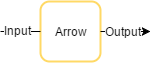
\includegraphics{images/arrow}
\vfill
%	\caption{Schematic depiction of an Arrow.}
%\label{fig:arrow-sch}
}
\parbox[c][17em]{0.49\linewidth}{%
\vfill
\centering
	{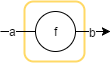
\includegraphics[scale=0.6]{images/arr}}
	{\includegraphics[scale=0.6]{images/compose}}
	{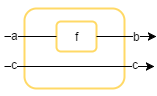
\includegraphics[scale=0.6]{images/first}}
\vfill
%\caption{Schematic depiction of |Arrow| combinators |arr|, |>>>| and |first|.}
%\label{fig:arrows-viz}
}
\caption{Schematic depiction of  an Arrow (left) and its basic
  combinators |arr|, |>>>| and |first| (right).}
\label{fig:arrow-sch}
\label{fig:arrows-viz}
\end{figure}

\subsection{Arrows}
\label{sec:arrows}
Arrows were introduced by \citet{HughesArrows} as a general interface for computation. An Arrow |arr a b| represents  a computation that converts an input |a| to an output |b|. This is defined in the |Arrow| type class shown in Fig.~\ref{fig:ArrowDefinition}.
%
To lift an ordinary function to an Arrow, |arr| is used, analogous to the monadic |return|. Similarly, the composition operator |>>>| is analogous to the monadic composition |>>=| and combines two arrows |arr a b| and |arr b c| by \enquote{wiring} the outputs of the first to the inputs to the second to get a new arrow |arr a c|. Lastly, the |first| operator takes the input Arrow |arr a b| and converts it into an arrow on pairs |arr (a, c) (b, c)| that leaves the second argument untouched. It allows us to to save input across arrows. Figure~\ref{fig:arrows-viz} shows a graphical representation of these basic Arrow combinators.
The most prominent instances of this interface are regular functions |(->)|
and the Kleisli type (Fig.~\ref{fig:ArrowDefinition}), which wraps monadic functions, e.g.  |a -> m b| (with |m| being a Monad).

\begin{figure}[h]
	\centering
	\begin{tabular}{cc}
		% \subcaptionbox
{\label{t1}}{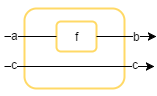
\includegraphics[width = 1.5in]{images/first}} &
		% \subcaptionbox
{\label{fig:secondImg}}{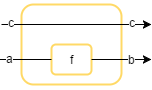
\includegraphics[width = 1.5in]{images/second}} \\
|first| & |second| \\
\midrule
		% \subcaptionbox
{}{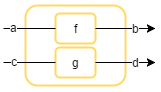
\includegraphics[width = 1.5in]{images/starstarstar}} &
		% \subcaptionbox
{}{\includegraphics[width = 1.5in]{images/andandand}}\\
|(***)|\label{fig:***Img} & |(&&&)| \label{fig:&&&Img} \\
	\end{tabular}
	\caption{Visual depiction of syntactic sugar for Arrows.}
	\label{fig:syntacticSugarArrows}
\end{figure}
Hughes also defined some syntactic sugar (Fig.~\ref{fig:syntacticSugarArrows}): |second|, |***| and |&&&|. 
|second| is the mirrored version of |first| (Appendix~\ref{utilfns}).
|***| combines |first| and |second| to handle two inputs in one arrow, and is defined as follows:
% \begin{figure}[h]
\begin{code}
(***) :: Arrow arr => arr a b -> arr c d -> arr (a, c) (b, d)
f *** g = first f >>> second g
\end{code}
% \caption{The (***) combinator}
% \label{fig:***}
% \end{figure}
The |&&&| combinator, which constructs an Arrow that outputs two different values like |***|, but takes only one input, is:
% \begin{figure}[h]
\begin{code}
(&&&) :: Arrow arr => arr a b -> arr a c -> arr a (b, c)
f &&& g = arr (\a -> (a, a)) >>> (f *** g)
\end{code}
% \caption{The (\&\&\&) combinator}
% \label{fig:&&&}
% \end{figure}
A~first short example given by Hughes on how to use arrows is addition with arrows:
%|add| over arrows, which can be seen in Fig.~\ref{fig:addArrows}.
% \begin{figure}[h]
\begin{code}
add :: Arrow arr => arr a Int -> arr a Int -> arr a Int
add f g = (f &&& g) >>> arr (\(u, v) -> u + v)
\end{code}
% \caption{Add over arrows}
% \label{fig:addArrows}
% \end{figure}
% The benefit of using the |Arrow| typeclass is that any type which is shown to be an arrow can be used in conjunction with this newly created |add| combinator. Even though this example is quite simple, the power of the arrow interface immediately is clear: If a type is an arrow, it can automatically used together with every library that works on arrows. Compared to simple Monads, this enables us to write code that is more extensible, without touching the internals of the specific arrows.
% \\\\
% \textit{Note: In the definitions Hughes gave in his paper, the notation |a b c| for an arrow from |b| to |c| is used. We use the equivalent definition |arr a b| for an arrow from |a| to |b| instead, to make it easier to find the arrow type in type signatures.}
%

The more restrictive interface of Arrows allows for more elaborate composition and transformation combinators---a Monad can be \emph{anything}, an Arrow is a process of doing something, a \emph{computation}. This is exactly one of the key challenges in parallel computing.


%%% Local Variables:
%%% mode: latex
%%% TeX-master: "main"
%%% End:

	\section{Background}
\label{sec:background}
\subsection{Short introduction to parallel Haskells}
There are already several ways to write parallel programs in Haskell. As we will base our parallel arrows on existing parallel Haskells, we will now give a short introduction to the ones we use as backends in this paper.

In its purest form, parallel computation (on functions) can be looked at as the execution of some functions \inlinecode{a -> b} in parallel:

\begin{figure}[h]
%\begin{lstlisting}[frame=htrbl]
\begin{code}
parEvalN :: [a -> b] -> [a] -> [b]
\end{code}
%\end{lstlisting}
\caption{parEvalN's type signature}
\label{fig:parEvalNTypeSig}
\end{figure}
\begin{figure}[h]
	\includegraphics[scale=0.7]{images/parEvalN}
	\caption{Schematic illustration of parEvalN}
	\label{fig:parEvalN}
\end{figure}
\olcomment{make them to real figures? with environment, reference and such?}
Before we go into detail on how we can use this idea of parallelism for parallel Arrows, as a short introduction to parallelism in Haskell we will now implement \inlinecode{parEvalN} with several different parallel Haskells.

\subsubsection{Multicore Haskell}
Multicore Haskell \cite{Marlow2009,Trinder1999} is way to do parallel processing found in standard GHC.\footnote{Multicore Haskell on Hackage is available under \url{https://hackage.haskell.org/package/parallel-3.2.1.0}, compiler support is integrated in the stock GHC.} It ships with parallel evaluation strategies \cite{Trinder1998a,Marlow2010} for several types which can be applied with \inlinecode{using :: a -> Strategy a -> a}. For \inlinecode{parEvalN} this means that we can just apply the list of functions \inlinecode{[a -> b]} to the list of inputs \inlinecode{[a]} by zipping them with the application operator \inlinecode{\$}. We then evaluate this lazy list \inlinecode{[b]} according to a \inlinecode{Strategy [b]} with the \inlinecode{using :: a -> Strategy a -> a} operator. We construct this strategy with \inlinecode{parList :: Strategy a -> Strategy [a]} and \inlinecode{rdeepseq :: NFData a => Strategy a} where the latter is a strategy which evalutes to normal form. To ensure that programs that use \inlinecode{parEvalN} have the correct evaluation order, we annotate the computation with \inlinecode{pseq :: a -> b -> b} which forces the compiler to not reorder multiple \inlinecode{parEvalN} computations. This is particularly necessary in circular communication topologies like in the \inlinecode{torus} or \inlinecode{ring} skeleton that we will see in chapter \ref{sec:topology-skeletons} which resulted in deadlock scenarios when executed without \inlinecode{pseq} during testing for this paper.

\begin{lstlisting}[frame=htrbl]
parEvalN :: (NFData b) => [a -> b] -> [a] -> [b]
parEvalN fs as = let bs = zipWith ($) fs as in
	(bs `using` parList rdeepseq) `pseq` bs
\end{lstlisting}
\begin{figure}[h]
	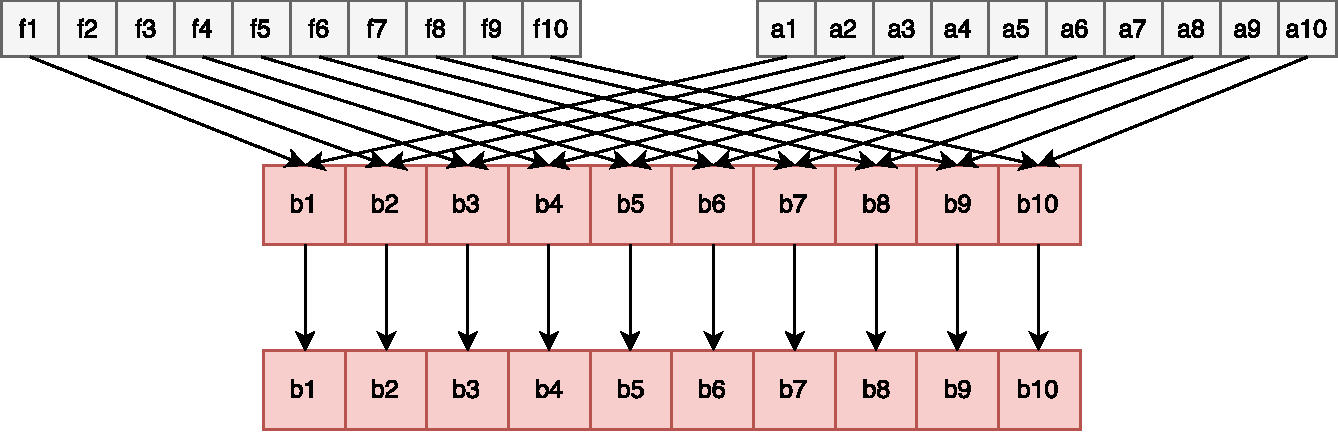
\includegraphics[scale=0.5]{images/parEvalNMulticore}
	\caption{Dataflow of the Multicore Haskell parEvalN version}
\end{figure} %$ %% formatting

\subsubsection{ParMonad}
The \inlinecode{Par} monad\footnote{It can be found in the \texttt{monad-par} package on hackage under \url{https://hackage.haskell.org/package/monad-par-0.3.4.8/}.} introduced by \citet{monad_par_paper_2011}, is a monad designed for composition of parallel programs.


Our parallel evaluation function \inlinecode{parEvalN} can be defined by zipping the list of \inlinecode{[a -> b]} with the list of inputs \inlinecode{[a]} with the application operator \inlinecode{\$} just like with Multicore Haskell. Then, we map over this not yet evaluated lazy list of results \inlinecode{[b]} with \inlinecode{spawnP :: NFData a => a -> Par (IVar a)} to transform them to a list of not yet evaluated forked away computations \inlinecode{[Par (IVar b)]}, which we convert to \inlinecode{Par [IVar b]} with \inlinecode{sequenceA}. We wait for the computations to finish by mapping over the \inlinecode{IVar b}'s inside the \inlinecode{Par} monad with \inlinecode{get}. This results in \inlinecode{Par [b]}. We finally execute this process with \inlinecode{runPar} to finally get \inlinecode{[b]} again.

\textbf{\textcolor{red}{explain problems with laziness here. Problems with torus}}

\begin{lstlisting}[frame=htrbl]
parEvalN :: (NFData b) => [a -> b] -> [a] -> [b]
parEvalN fs as = runPar $ 
	(sequenceA $ map (spawnP) $ zipWith ($) fs as) >>= mapM get
\end{lstlisting}
\begin{figure}[h]
	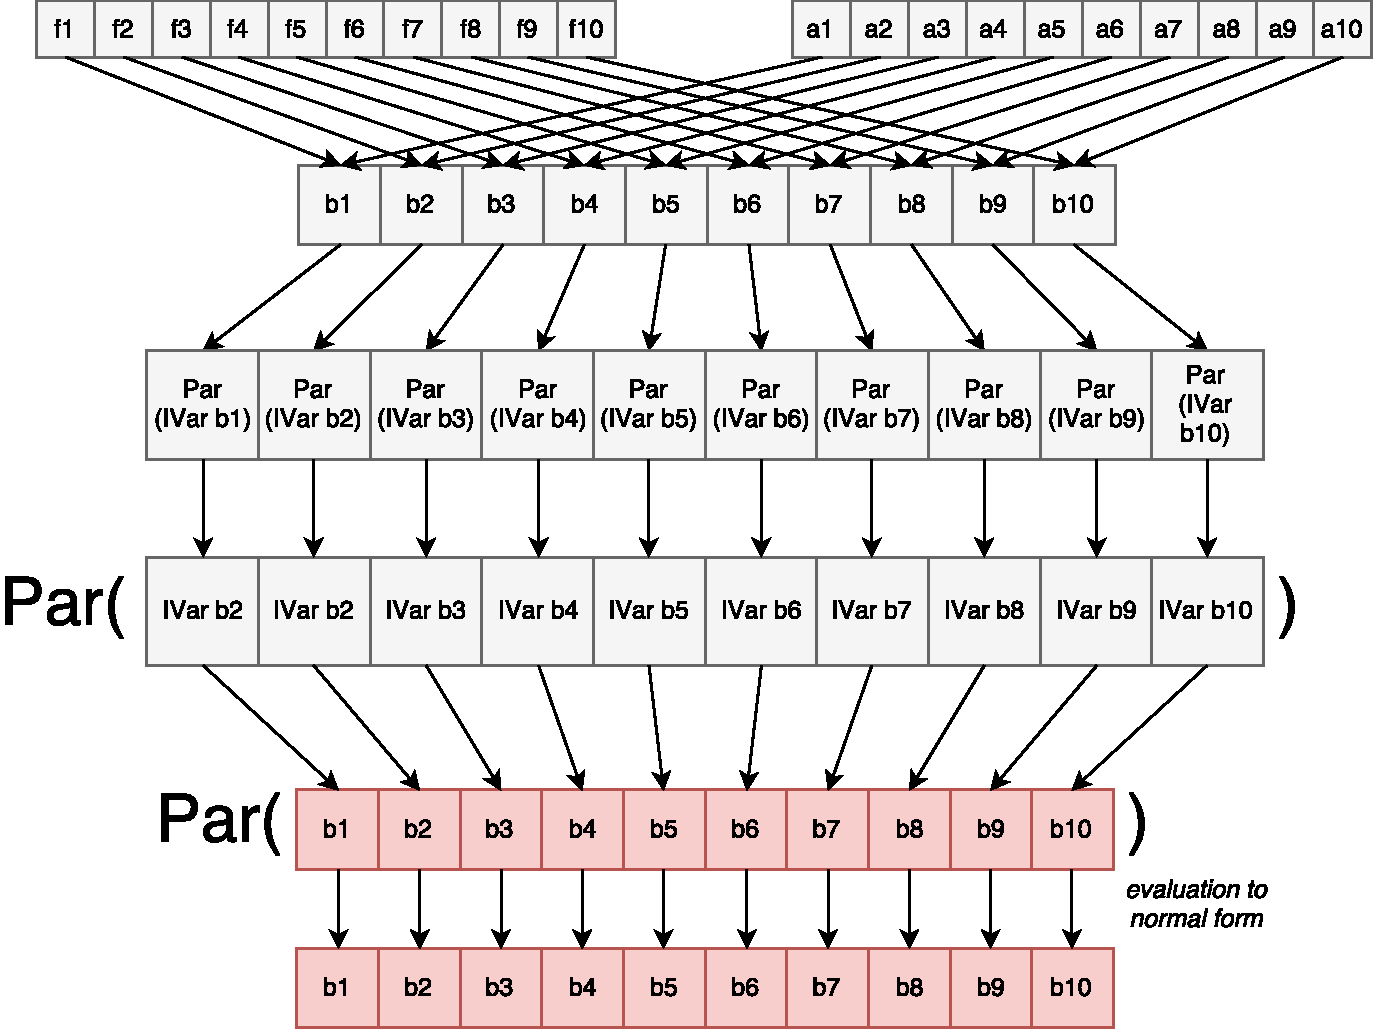
\includegraphics[scale=0.5]{images/parEvalNParMonad}
	\caption{Dataflow of the Par Monad parEvalN version}
\end{figure}

\subsubsection{Eden}
Eden \cite{eden,Loogen2012} is a parallel Haskell for distributed memory and comes with a MPI and a PVM backends.\footnote{See also \url{http://www.mathematik.uni-marburg.de/~eden/} and \url{https://hackage.haskell.org/package/edenmodules-1.2.0.0/}.} This means that it works on clusters as well so it makes sense to have a Eden-based backend for our new parallel Haskell flavour.

Eden was designed to work on clusters, but with a further simple backend it operates on multicores. However, in contrast to many other parallel Haskells, in Eden each process has its own heap. This seems to be a waste of memory, but with distributed programming paradigm and individual GC per process, Eden yields good performance results also on multicores \cite{arcs-dc,aswad2009low}.

While Eden also comes with a monad \inlinecode{PA} for parallel evaluation, it also ships with a completely functional interface that includes
%\\
%\inlinecode{spawnF :: (Trans a, Trans b) => [a -> b] -> [a] -> [b]}.
%\\
a \inlinecode{spawnF} function that
%This 
allows us to define \inlinecode{parEvalN} directly:

\begin{lstlisting}[frame=htrbl]
parEvalN :: (Trans a, Trans b) => [a -> b] -> [a] -> [b]
parEvalN = spawnF 
\end{lstlisting}
\begin{figure}[h]
	\includegraphics[scale=0.5]{images/parEvalNEden}
	\caption{Dataflow of the Eden parEvalN version}
\end{figure}

\paragraph{Eden TraceViewer.}
To comprehend the efficiency and the lack thereof in a parallel program, an inspection of its execution is extremely helpful. While some large-scale solutions exist \cite{Geimer2010}, the parallel Haskell community mainly utilises the tools Threadscope \cite{Wheeler2009} and Eden TraceViewer\footnote{See ..... on hackage for the last available version of Eden TraceViewer. There was an effort to implement the TraceViewer using modern web technologies \cite{traceviewer-web}.} \cite{Berthold2007a}. In the next sections we will present some \emph{traces}, the post-mortem process diagrams of Eden processes and their activity.

In a trace, the $x$ axis shows the time, the $y$ axis enumerates the machines and processes. A~trace shows a running process in green, a blocked process is red. If the process is \enquote{runnable}, \ie it may run, but does not, it is yellow. The typical reason for then is GC. An inactive machine where no processes are started yet, or all are already terminated, is shows as a blue bar. A~comminication from one process to another is represented with a black arrow. A~stream of communications, \eg a transmitted list is shows as a dark shading between sender and receiver processes.

\olcomment{show example trace or refer to a trace in later figures}


%%% Local Variables:
%%% mode: latex
%%% TeX-master: "main"
%%% End:

	\section{Parallel Arrows}
We have seen what Arrows are and how they can be seen as a general interface to computation. In the following section we will discuss how Arrows can also be seen as a general interface not only to computation, but to \textbf{parallel computation} as well. We start by introducing the interface and explaining the reasonings behind it. Then, we discuss some implementations using exisiting parallel Haskells. Finally, we explain why using Arrows for expressing parallelism is beneficial.
\subsection{The ArrowParallel interface}
In its purest form, parallel computation (on functions) can be looked at as the execution of some functions \code{a -> b} in parallel:
\begin{lstlisting}[frame=htrbl]
parEvalN :: [a -> b] -> [a] -> [b]
\end{lstlisting}
Translating this into arrow terms gives us a new operator \code{parEvalN} that lifts a list of arrows \code{[arr a b]} to a parallel arrow \code{arr [a] [b]} (This combinator is similar to our utility function listApp, but does parallel instead of serial evaluation).
\begin{lstlisting}[frame=htrbl]
parEvalN :: (Arrow arr) => [arr a b] -> arr [a] [b]
\end{lstlisting}
With this definition of \code{parEvalN}, parallel execution can be looked at as yet another arrow combinator. But as the implementation may differ depending on the actuall type of the arrow \code{arr} and we want this to be an interface for different backends, we have to introduce the new typeclass \code{ArrowParallel} to host this combinator.
\begin{lstlisting}[frame=htrbl]
class Arrow arr => ArrowParallel arr a b where
	parEvalN :: [arr a b] -> arr [a] [b]
\end{lstlisting}
Sometimes parallel Haskells require additional configuration parameters for information about the execution environment. This is why we also introduce an additional \code{conf} parameter to the function. We also do not want \code{conf} to be of a fixed type, as the configuration parameters can differ for different instances of \code{ArrowParallel}, so we add it to the type signature of the typeclass as well.
\begin{lstlisting}[frame=htrbl]
class Arrow arr => ArrowParallel arr a b conf where
	parEvalN :: conf -> [arr a b] -> arr [a] [b]
\end{lstlisting}
We don't require the conf parameter in every implementation. If it is not needed, we usually want to allow the \code{conf} type parameter to be of any type and don't even evaluate it by blanking it in the type signature of the implemented \code{parEvalN} as we will see in the implementation sections.

\subsection{Multicore Haskell}
The Multicore Haskell implementation of this class is straightforward using listApp from \ref{utilfns} combined with the \code{using} operator from Multicore Haskell.
\begin{lstlisting}[frame=htrbl]
instance (NFData b, ArrowApply arr, ArrowChoice arr) =>
	ArrowParallel arr a b conf where
		parEvalN _ fs = listApp fs >>> arr (flip using $ parList rdeepseq)
\end{lstlisting}
We hardcode the \code{parList rdeepseq} strategy here as in this context it is the only one making sense as we usually want the output list to be fully evaluated to its normal form.

\subsection{ParMonad}
The ParMonad implementation makes use of Haskells laziness and ParMonad's \code{spawnP :: a -> Par (IVar a)} function which forks away the computation of a value and returns an IVar containing the result in the Par monad.
\\\\
We therefore apply each function to its corresponding input value with \code{app} and then fork the computation away with \code{arr spawnP} inside a \code{zipWithArr} call. This yields a list \code{[Par (IVar b)]}, which we then convert into \code{Par [IVar b]} with \code{arr sequenceA}. In order to wait for the computation to finish, we map over the \code{IVar}s inside the ParMonad with \code{arr (>>= mapM get)}. The result of this operation is a \code{Par [b]} from which we can finally remove the monad again by running \code{arr runPar} to get our output of \code{[b]}.
\begin{lstlisting}[frame=htrbl]
instance (NFData b, ArrowApply arr, ArrowChoice arr) =>
	ArrowParallel arr a b conf where
		parEvalN _ fs = 
			(arr $ \as -> (fs, as)) >>>
			zipWithArr (app >>> arr spawnP) >>>
			arr sequenceA >>>
			arr (>>= mapM get) >>>
			arr runPar
\end{lstlisting}

\subsection{Eden}
For the Multicore and ParMonad implementation we could use general implementations that just required the \code{ArrowApply} and \code{ArrowChoice} typeclasses. With Eden this is not the case as we can only spawn a list of functions and we cannot extract simple functions out of arrows. While we could still manage to have only one class in the module by introducing a typeclass like
\begin{lstlisting}[frame=htrbl]
class (Arrow arr) => ArrowUnwrap arr where
	arr a b -> (a -> b)
\end{lstlisting}
we don't do this in this paper, as this seems too hacky. For now, we just implement \code{ArrowParallel} for normal functions
\begin{lstlisting}[frame=htrbl]
instance (Trans a, Trans b) => ArrowParallel (->) a b conf where
parEvalN _ fs as = spawnF fs as
\end{lstlisting}
and the Kleisli type.
\begin{lstlisting}[frame=htrbl]
instance (Monad m, Trans a, Trans b, Trans (m b)) =>
	ArrowParallel (Kleisli m) a b conf where
parEvalN conf fs =
	(arr $ parEvalN conf (map (\(Kleisli f) -> f) fs)) >>>
	(Kleisli $ sequence)
\end{lstlisting}

\subsection{HdpH}

\subsection{Benefits of parallel Arrows}
We have seen that we can wrap parallel Haskells inside of the \code{ArrowParallel} interface, but why do we abstract parallelism this way and what does this approach do better than the other parallel Haskells?
\begin{itemize}
	\item \textbf{Arrow API benefits}:
	With the \code{ArrowParallel} typeclass we do not lose any benefits of using arrows as \code{parEvalN} is just yet another arrow combinator. The resulting arrow can be used in the same way its serial version can be used. This is a big advantage of this approach, especially compared to the monad solutions as all arrow combinators will continue to work instead of requiring special ones for each parallel monad.
	\item \textbf{Abstraction}:
	With the \code{ArrowParallel} typeclass, we abstracted all parallel implementation logic away from the business logic. This gives us the beautiful situation of being able to write our code against the interface the typeclass gives us without being bound to any parallel Haskell. So as an example, during development, we can run the code on the simple Multicore version and afterwards deploy it on a cluster using an Eden built, by just swapping out the actual \code{ArrowParallel} instance.
\end{itemize}

	%\section{Utility Functions}\label{utilfns}
\subsection{mapArr}
The mapArr combinator lifts any arrow \code{arr a b} to an arrow \code{arr [a] [b]} \cite{programming_with_arrows},
\begin{lstlisting}[frame=htrbl]
mapArr :: ArrowChoice arr => arr a b -> arr [a] [b]
mapArr f =
	arr listcase >>>
	arr (const []) ||| (f *** mapArr f >>> arr (uncurry (:)))
	where
		listcase [] = Left ()
		listcase (x:xs) = Right (x,xs)
\end{lstlisting}
with
\begin{lstlisting}[frame=htrbl]
(|||) :: ArrowChoice arr a c -> arr b c -> arr (Either a b) c
\end{lstlisting}
%It takes two arrows \code{arr a c} and \code{arr b c} and combines them into a new arrow \code{arr (Either a b) c} which pipes all \code{Left a}'s to the first arrow and all \code{Right b}'s to the second arrow.
\frbreak

\subsection{zipWithArr \& listApp}
zipWithArr lifts any arrow \code{arr (a, b) c} to an arrow \code{arr ([a], [b]) [c]}:
\begin{lstlisting}[frame=htrbl]
zipWithArr :: ArrowChoice arr => arr (a, b) c -> arr ([a], [b]) [c]
zipWithArr f = (arr $ \(as, bs) -> zipWith (,) as bs) >>>
	mapArr f
\end{lstlisting}
listApp converts a list of arrows \code{[arr a b]} to a new arrow \code{arr [a] [b]}:
\begin{lstlisting}[frame=htrbl]
listApp :: (ArrowChoice arr, ArrowApply arr) =>
	[arr a b] -> arr [a] [b]
listApp fs = (arr $ \as -> (fs, as)) >>> zipWithArr app
\end{lstlisting}
with the \code{ArrowApply} that defines \code{app :: arr (arr a b, a) c}.

	\subsection{ArrowParallel Implementations}
\begin{frame}[fragile]{GpH}
\begin{lstlisting}[frame=htrbl]
data Conf a = Conf (Strategy a)

instance (ArrowChoice arr) =>
  ArrowParallel arr a b (Conf b) where
    parEvalN (Conf strat) fs =
        evalN fs >>>
        arr (withStrategy (parList strat))
\end{lstlisting}
\begin{center}
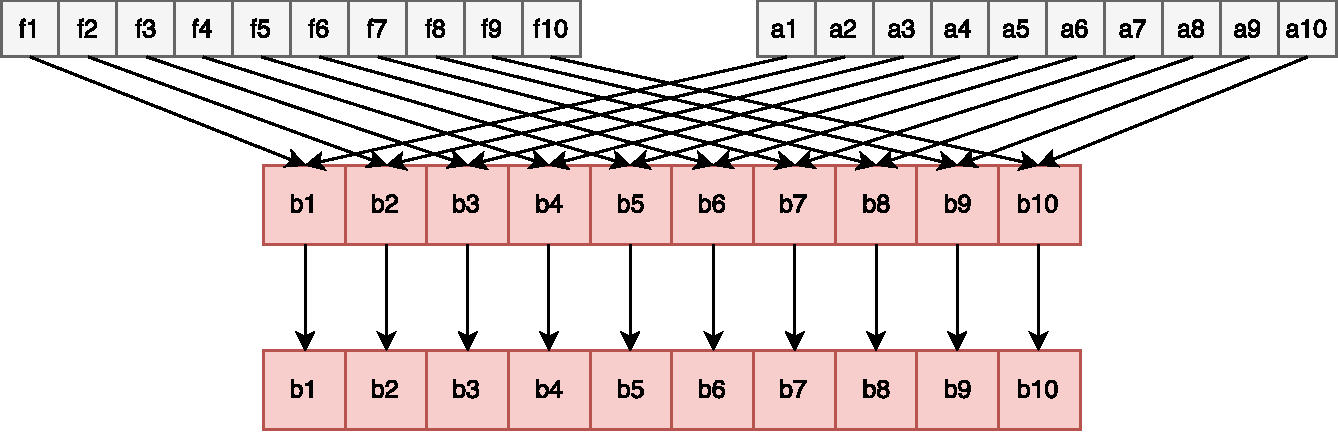
\includegraphics[scale=0.45]{images/parEvalNMulticore}
\end{center}
\end{frame}

\begin{frame}[fragile]{ParMonad}
\begin{lstlisting}[frame=htrbl]
type Strategy a = a -> Par (IVar a)
data Conf a = Conf (Strategy a)

instance (ArrowChoice arr) => ArrowParallel arr a b (Conf b) where
    parEvalN (Conf strat) fs =
        evalN (map (>>> arr strat) fs) >>>
        ...
\end{lstlisting}
\begin{center}
\includegraphics[scale=0.4]{images/parEvalNParMonad1}
\end{center}
\end{frame}

\begin{frame}[fragile]{ParMonad}
\begin{lstlisting}[frame=htrbl]
        ...
        arr sequenceA >>>
        arr (>>= mapM Control.Monad.Par.get) >>>
        arr runPar
\end{lstlisting}
\begin{center}
\includegraphics[scale=0.4]{images/parEvalNParMonad2}
\end{center}
\end{frame}


\begin{frame}[fragile]{Eden problems}
For Eden we need separate implementations.\\~\\
This is because of \code{spawnF} only supporting functions \lstinline{(->)}:
\begin{lstlisting}[frame=htrbl]
spawnF :: (Trans a, Trans b) => [a -> b] -> [a] -> [b]
\end{lstlisting}
\pause
Hacky alternative:
\begin{lstlisting}[frame=htrbl]
class (Arrow arr) => ArrowUnwrap arr where
    arr a b -> (a -> b)
\end{lstlisting}
\end{frame}

\begin{frame}[fragile]{Eden implementation - Functions}
Straightforward:
\begin{lstlisting}[frame=htrbl]
data Conf = Nil

instance (Trans a, Trans b) => ArrowParallel (->) a b conf where
	parEvalN _ = spawnF
\end{lstlisting}
\begin{center}
\includegraphics[scale=0.5]{images/parEvalNEden}
\end{center}
\end{frame}

\begin{frame}[fragile]{Eden implementation - Kleisli}
Implementation for the Kleisli Type:
\begin{lstlisting}[frame=htrbl]
instance (ArrowParallel (->) a (m b) Conf,
  Monad m, Trans a, Trans b, Trans (m b)) =>
  ArrowParallel (Kleisli m) a b conf where
    parEvalN conf fs = 
      arr (parEvalN conf (map (\(Kleisli f) -> f) fs)) >>>
      Kleisli sequence
\end{lstlisting}
\begin{center}
\includegraphics[scale=0.5]{images/parEvalNEden}
\end{center}
\end{frame}
	\subsection{Map Skeletons}
\begin{frame}[fragile]{Map Skeletons (1)}
parEvalN, but \textbf{chunky}:
\begin{lstlisting}[frame=htrbl]
parEvalNLazy :: conf -> ChunkSize -> [arr a b] -> arr [a] [b]
\end{lstlisting}
\begin{center}
\includegraphics[scale=0.5]{images/parEvalNLazy}
\end{center}
parallel evaluation of \textbf{different typed functions}:
\begin{lstlisting}[frame=htrbl]
parEval2 :: conf -> arr a b -> arr c d -> arr (a, c) (b, d)
\end{lstlisting}
\begin{center}
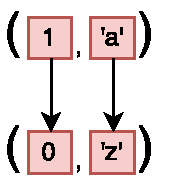
\includegraphics[scale=0.5]{images/parEval2}
\end{center}
\end{frame}
\begin{frame}[fragile] {Map Skeletons (2)}
map, but in \textbf{parallel}:
\begin{lstlisting}[frame=htrbl]
parMap :: conf -> arr a b -> arr [a] [b]
\end{lstlisting}
\begin{center}
\includegraphics[scale=0.5]{images/parMap}
\end{center}
parMap, but \textbf{chunky}:
\begin{lstlisting}[frame=htrbl]
parMapStream :: conf -> ChunkSize -> arr a b -> arr [a] [b]
\end{lstlisting}
\begin{center}
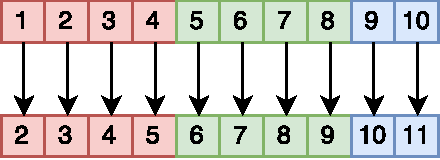
\includegraphics[scale=0.5]{images/parMapStream}
\end{center}
\end{frame}
\begin{frame}[fragile]{Map Skeletons (3)}
parMap, but with \textbf{workload distribution}:
\begin{lstlisting}[frame=htrbl]
farm :: conf -> NumCores -> arr a b -> arr [a] [b]
\end{lstlisting}
\begin{center}
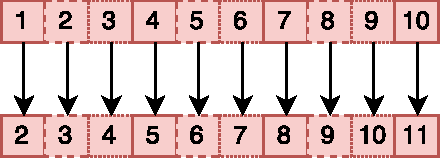
\includegraphics[scale=0.5]{images/farm}
\end{center}
farm, but \textbf{chunky}:
\begin{lstlisting}[frame=htrbl]
farmChunk ::
	conf -> ChunkSize -> NumCores -> arr a b-> arr [a] [b]
\end{lstlisting}
\begin{center}
\includegraphics[scale=0.5]{images/farmChunk}
\end{center}
\end{frame}
	\subsubsection{Syntactic Sugar} \label{syntacticSugar}
For basic arrows, we have the \inlinecode{(***)} combinator (Fig.~\ref{fig:***Img},~\ref{fig:***}) which allows us to combine two arrows \inlinecode{arr a b} and \inlinecode{arr c d} into an arrow \inlinecode{arr (a, c) (b, d)} which does both computations at once. This can easily be translated into a parallel version \inlinecode{(|***|)} (Fig.~\ref{fig:|***|}) with the use of \inlinecode{parEval2}, but for this we require a backend which has an implementation that does not require any configuration (hence the \inlinecode{()} as the conf parameter in Fig.~\ref{fig:|***|}).
\begin{figure}[h]
\begin{lstlisting}[frame=htrbl]
(|***|) :: (ArrowChoice arr, ArrowParallel arr (Either a c) (Either b d) ())) =>
	arr a b -> arr c d -> arr (a, c) (b, d)
(|***|) = parEval2 ()
\end{lstlisting}
\caption{Definition of (|***|) - the parallel version of (***)}
\label{fig:|***|}
\end{figure}
% With this we can analogously to the serial \inlinecode{&&&}
We define the parallel \inlinecode{(|\&\&\&|)} (Fig.~\ref{fig:|&&&|}) in a similar manner to its sequential pendant \inlinecode{(\&\&\&)} (Fig.~\ref{fig:&&&Img},~\ref{fig:&&&}).
\begin{figure}[h]
\begin{lstlisting}[frame=htrbl]
(|&&&|) :: (ArrowChoice arr, ArrowParallel arr (Either a a) (Either b c) ()) =>
	arr a b -> arr a c -> arr a (b, c)
(|&&&|) f g = (arr $ \a -> (a, a)) >>> f |***| g
\end{lstlisting} % $ %% formatting
\caption{Definition of (|\&\&\&|) - the parallel version of (\&\&\&)}
\label{fig:|&&&|}
\end{figure}
	\section{Performance results}
\label{sec:benchmarks}

\newcommand{\rmtest}{Rabin--Miller test\xspace}
\newcommand{\sudokutest}{Sudoku\xspace}
\newcommand{\jacobitest}{Jacobi sum test\xspace}
\newcommand{\torustest}{Gentleman\xspace}
\newlength{\plotwidthSMP}
\setlength{\plotwidthSMP}{0.39\textwidth}
\newlength{\plotwidthDist}
\setlength{\plotwidthDist}{0.6\textwidth}


\newcommand{\performanceplot}[7]{
\begin{tikzpicture}
\begin{axis}[title={#1},
title style={align=center},
scale only axis, width=#7,
xlabel=Threads,
%xtick=data,
xtick distance=#4,
ylabel=Time (s),
ylabel near ticks,
minor tick num=2,
grid=major,
legend entries={#2},
legend style={at={(0.99,0.99)},anchor=north east},
max space between ticks=50pt,
grid style={line width=.1pt, draw=gray!10},
major grid style={line width=.2pt,draw=gray!50},
xmin=-1,
xmax=#6]
#5
\end{axis}
\end{tikzpicture}
}

\newcommand{\performancediffplot}[8]{
\begin{tikzpicture}
\begin{axis}[title={#1},
title style={align=center},
scale only axis, width=#8,
xlabel=Threads,
%xtick=data,
ytick distance=#6,
xtick distance=#4,
minor tick num=9,
ylabel=Absolute time difference (s),
ylabel near ticks,
grid=both,
legend entries={#2},
legend style={at={(0.99,0.99)},anchor=north east},
max space between ticks=50pt,
grid style={line width=.1pt, draw=gray!10},
major grid style={line width=.2pt,draw=gray!50},
xmin=-1,
xmax=#7]
#5
\end{axis}
\end{tikzpicture}
}

\newcommand{\speedupplot}[7]{
\begin{tikzpicture}
\begin{axis}[title={#1},
title style={align=center},
scale only axis, width=#7,
xlabel=Threads,
%xtick=data,
%ytick=data,
xtick distance=#4,
ytick distance=#4,
ylabel=Speedup,
ylabel near ticks,
grid=major,
legend entries={linear, #2},
legend style={at={(0.01,0.99)},anchor=north west},
max space between ticks=50pt,
grid style={line width=.1pt, draw=gray!10},
major grid style={line width=.2pt,draw=gray!50},
ymin=-1,
xmin=-1,
ymax=#6,
xmax=#6]
\addplot [domain=0:#3, no markers,dotted,thick]{x};
#5
\end{axis}
\end{tikzpicture}
}

\newcommand{\speedupdiffplot}[7]{
\begin{tikzpicture}
\begin{axis}[title={#1},
title style={align=center},
scale only axis, width=#7,
xlabel=Threads,
%xtick=data,
xtick distance=#4,
ytick distance=0.5,
ylabel=Absolute speedup difference,
ylabel near ticks,
grid=major,
legend entries={#2},
legend style={at={(0.99,0.99)},anchor=north east},
max space between ticks=50pt,
grid style={line width=.1pt, draw=gray!10},
major grid style={line width=.2pt,draw=gray!50},
xmin=-1,
xmax=#6]
#5
\end{axis}
\end{tikzpicture}
}

\subsection{Hardware}

We have tested our parallel DSL and algorithmic skeletons implemented
in it. Benchmarks were conducted both in a shared and in a distributed
memory setting. All benchmarks were done on the ``Glasgow grid'', consisting of
16 machines with 2 Intel\SymbReg~Xeon\SymbReg~E5-2640 v2 and 64 GB of DDR3 RAM each. Each processor has 8 cores and 16 (hyper-threaded) threads with a base frequency of 2 GHz and a turbo frequency of 2.50 GHz. This results in a total of 256 cores and 512 threads for the whole cluster. The operating system was Ubuntu 14.04 LTS with Kernel 3.19.0-33. Non-surprisingly, we found that hyper-threaded 32 cores do not behave in the same manner as real 16 cores (numbers here for a single machine). We disregarded the hyper-threading ability in most of the
cases.

We used a single node with 16 real cores as a shared memory testbed
and the whole grid with 256 real cores as a device to test our
distributed memory software.

\subsection{Test programs}

We used multiple tests that originated from different
sources. Most of them are parallel mathematical computations, initially
implemented in Eden. Table~\ref{tab:benches} summarises.

\begin{table}
\caption{The benchmarks we use in this paper.}
\label{tab:benches}
\centering
%% something was wrong with separators in table
\renewcommand{\tabcolsep}{0.5em}
\begin{tabular}{lccll}
\toprule
Name & Area & Type & Origin & Citation \\
\midrule
\rmtest & Mathematics & |parMap+reduce| & Eden & \citet{Lobachev2012}\\
\jacobitest & Mathematics & |workpool+reduce| & Eden & \citet{Lobachev2012}\\
\torustest & Mathematics & |torus| & Eden & \citet{Eden:SkeletonBookChapter02}\\
\sudokutest & Puzzle & |parMap| & |Par| Monad & \citet{par-monad} 
\tablefootnote{actual code from: http://community.haskell.org/~simonmar/par-tutorial.pdf and https://github.com/simonmar/parconc-examples}\\
\bottomrule
\end{tabular}
\end{table}

\rmtest is a probabilistic primality test that iterates multiple (32--256 here)
``subtests''. Should a subtest fail, the input is definitely not a
prime. If all $n$ subtest pass, the input is composite with the
probability of $1/4^{n}$. 

Jacobi sum test or APRCL is also a primality test, that however,
guarantees the correctness of the result. It is probabilistic in the
sense that its run time is not certain. Unlike \rmtest, the subtests
of Jacobi sum test have very different durations. \citet{lobachev-phd}
discusses some optimisations of parallel APRCL. Generic parallel
implementations of \rmtest and APRCL were presented in \citet{Lobachev2012}.

``Gentleman'' is a standard Eden test program, developed
for their |torus| skeleton. It implements a parallel matrix
multiplication \citep{Gentleman1978}. We ported an Eden based version \citep{Eden:SkeletonBookChapter02} to PArrows.

A~parallel Sudoku solver was used by \citet{par-monad} to compare |Par| Monad
to GpH Haskell. We ported it to PArrows.



\subsection{What parallel Haskells run where}

The \ensuremath{\Conid{Par}} monad and GpH Haskell -- in its multicore version (\cite{Marlow2009}) --  can be executed on a shared
memory machines only. Although GpH is available on distributed memory
clusters, and newer distributed memory Haskells such as HdpH exist,
current support of distributed memory in PArrows is limited to
Eden. We used the MPI backend of Eden in a distributed memory
setting. However, for shared memory Eden features a ``CP'' backend
that merely copies the memory blocks between distributed heaps. In
this mode, Eden still operates in the ``nothing shared'' setting, but
is adapted better to multicore machines. We label this version of Eden
in the plots as ``Eden~CP''.



\subsection{Effect of hyper-threading}

The PArrows version of \rmtest on a single node of the Glasgow grid
showed almost linear speedup (Fig.~\ref{fig:bench-rm-sm}). The speedup
of 64-task PArrows/Eden at 16 real cores version was 13.65, the
efficiency was 85.3\%. However, if we increase the number of
requested cores to be 32 -- \ie if we use hyper-threading on 16 real
cores -- the speedup does not increase that well. It is merely 15.99
for 32 tasks with PArrows/Eden. It is worse for other backends.  As
for 64 tasks, we obtain the speedup of 16.12 with PArrows/Eden at 32
hyper-threaded cores and only 13.55 with PArrows/GpH. Efficiency is 50.4\% and 42.3\%, respectively. The Eden
version used here was Eden~CP, the \enquote{share nothing} SMP build.

In the distributed memory setting the same effect ensues. We obtain
plummeting speedup of 124.31 at 512 hyper-threaded cores, whereas it was
213.172 for 256 real cores. Apparently, hyper-threading in the Glasgow
grid fails to execute two parallel Haskell processes with full-fledged
parallelism. For this reason, we did not regard hyper-threaded cores in
our speedup plots in Figs.~\ref{fig:bench-rm-sm}--\ref{fig:sudokuSMBenchmark}.


% rm 11213 32 32-sm speedup eden: 15.993037587283924
% -"- multi: 15.09948017762912
% -"- par: 14.909092857846693

% -"- 64 32-sm speedup eden: 16.118040224478424
% -"- multi: 13.545304115702333
% -"- par: 15.155709987503396

\subsection{Benchmark results}

The difference between, say, PArrows with |Par| Monad backend and a
genuine |Par|
Monad benchmark is very small. To give an example, it is ~0.4\seconds in favour of PArrows for 16 cores (10.8\seconds vs. 11.2\seconds) and ~-0.8\seconds in favour of the |Par| monad for 8 cores (16.1\seconds vs. 16.9\seconds) for
the Sudoku benchmark in the shared memory setting. It is almost invisible in speedup and
(non shown) run time plots. We thus show only the results for the
PArrows-enabled versions.

To show that PArrows induce very small overhead in a distributed context as well, we compare the original Eden
versions of the benchmark to its PArrows-enabled counterpart in the \rmtest, \torustest and \jacobitest benchmarks. We plot execution time differences between measurements for
PArrows and the corresponding backend in a separate plot
(Figs.~\ref{fig:bench-rm-dist}--\ref{fig:torusBenchmark}). As an example, the differences range in
about 0.5\seconds for the execution time of 46\seconds on 256 cores
for distributed \rmtest with PArrows and Eden. For these comparisons, the plots show absolute
time differences that are not relative \wrt the total execution time.
Furthermore, the error bars ends were computed from point-wise maximum of both standard
deviations from both measurements for PArrows and non-PArrows
versions. These are the values provided by the |bench| package that we
used for bench-marking. We call a difference between two versions
significant when the border of the error bar of absolute time
difference is above or below zero. In other words: the time
difference is significant if it is above measurement error.

\subsubsection{\rmtest}\label{sec:rmtest}

\newcommand{\performanceSkelRMSM}[2]{
\performanceplot{Parallel run time of \rmtest \enquote{#2}}{Eden CP, GpH, |Par| Monad}{16}{4}{
\addplot+ [very thick] table [scatter, x="nCores", y="time", col sep=comma, mark=none,
smooth]{benchmarks/sm-rm/bench-sm-rm.bench.skelrm-parr-eden-cp-#1-#2.csv};
\addplot+ [very thick] table [scatter, x="nCores", y="time", col sep=comma, mark=none,
smooth]{benchmarks/sm-rm/bench-sm-rm.bench.skelrm-parr-mult-#1-#2.csv};
\addplot+ [very thick] table [scatter, x="nCores", y="time", col sep=comma, mark=none,
smooth]{benchmarks/sm-rm/bench-sm-rm.bench.skelrm-parr-par-#1-#2.csv};
}{17}{\plotwidthSMP}
}

\newcommand{\speedupSkelRMSM}[2]{
\speedupplot{Speedup of \rmtest \enquote{#2}}{Eden CP, GpH, |Par| Monad}{16}{4}{
\addplot+ [very thick] table [scatter, x="nCores", y="speedup", col sep=comma, mark=none,
smooth]{benchmarks/sm-rm/bench-sm-rm.bench.skelrm-parr-eden-cp-#1-#2.csv};
\addplot+ [very thick] table [scatter, x="nCores", y="speedup", col sep=comma, mark=none,
smooth]{benchmarks/sm-rm/bench-sm-rm.bench.skelrm-parr-mult-#1-#2.csv};
\addplot+ [very thick] table [scatter, x="nCores", y="speedup", col sep=comma, mark=none,
smooth]{benchmarks/sm-rm/bench-sm-rm.bench.skelrm-parr-par-#1-#2.csv};
}{17}{\plotwidthSMP}
}

\newcommand{\speedupSkelRMDist}[4]{
\speedupplot{Speedup of \rmtest \enquote{#1 #2}}{PArrows}{256}{#3}{
% \addplot [mark=*,very thick] table [scatter, x="nCores", y="speedup", col sep=comma, mark=none,
% smooth]{benchmarks/distributed-rm/bench-distributed.bench.skelrm-parrows-11213-#2.csv};
\addplot [mark=*,very thick,blue] table [scatter, x="nCores", y="speedup", col sep=comma, mark=none,
smooth]{benchmarks/distributed-rm/bench-distributed.bench.skelrm-parrows-#1-#2.csv};
% \addplot table [scatter, x="nCores", y="speedup", col sep=comma, mark=none,
% smooth]{benchmarks/distributed-rm/bench-distributed.bench.skelrm-eden-#1-#2.csv};
}{#4}{\plotwidthDist}
}

\newcommand{\performanceSkelRMDistDiff}[5]{
\performancediffplot{Run time differences\\for \rmtest \enquote{#1 #2}}{(Eden $-$ PArrows)}{256}{#3}{
\addplot+[mark=*,very thick,error bars/.cd,
    y dir=both,y explicit] table [x="nCores", y="time", y error="max stddev", col sep=comma, mark=dots,
smooth]{benchmarks/distributed-rm/#1-#2-diff.csv};
}{#4}{#5}{\plotwidthDist}
}

\begin{figure}
%\centering
%\performanceSkelRMSM{11213}{64}\hfill%
{\speedupSkelRMSM{11213}{32}}\hfill%
{\speedupSkelRMSM{11213}{64}}
\caption{Relative speedup of \rmtest on a multicore machine. We used the same PArrows-based implementation with
  different backends on the same hardware. Measurements were performed on a single node of the Glasgow
  grid; it has 16 real cores. Input was $2^{11213}-1$, we used 32 (left) or 64 (right)
  tasks. The
  closer to linear speedup the better.}
\label{fig:bench-rm-sm}
\end{figure}

\begin{figure}
\centering
%\performanceSkelRMDist{44497}{256}{32,64,128,256,512}{544}
%
{\speedupSkelRMDist{44497}{256}{32}{272}\label{subfig:rm-dist-a}}%
%\hfill%
{\performanceSkelRMDistDiff{44497}{256}{32}{0.5}{272}\label{subfig:rm-dist-b}}
\caption{Parallel performance of \rmtest on the Glasgow grid
  consisting of 256 cores. Input was $2^{44497}-1$, we used 256
  tasks. The top plot shows absolute speedup in a distributed memory setting. The
  closer to linear speedup the better. Time
  (and hence speedup) measurements for PArrows with Eden backend and
  Eden almost coincide. Hence, bottom plot shows
absolute time differences for this benchmark. The
higher the value, the better for PArrows\olcomment{CHECKME}.}
\label{fig:bench-rm-dist}
\end{figure}

\olcomment{THE ACTUAL TEXT IS MISSING. What do we see in the plots?
  Why is it good?}
The multicore version of our parallel \rmtest benchmark is depicted in
Figure~\ref{fig:bench-rm-sm}. We executed the test with 32 and 64
tasks. The plot shows the PArrows-enabled versions with corresponding backends.
The performance of PArrows/Eden~CP in shared memory is slightly better than
for SMP variants such as PArrows/GpH and PArrows/|Par|
Monad but most of the time the performance is still comparable with the GpH backend performing slightly worse than the other two in terms of speedup.

Comparing the PArrows version of the \rmtest with the original from Eden with the MPI backend in a distributed memory setting, we see an almost linear speedup of
\rmtest with 256 tasks and input $2^{44497}-1$ in both versions. The sequential run time
was computed as the mean of three consecutive executions on a single
core---the single run took two hours 43 minutes. The difference between
PArrows/Eden and Eden almost always lies inside the error bar of
the measurement.

%As the PArrows version uses Eden in the backend, these numbers suggest that there is no real performance difference between using PArrows or Eden for this task as they trade blows in this benchmark. Additionally, PArrows with an Eden-based backend performing better than what it is based upon suggests that any difference in runtime between the two is more of an anomaly than a real difference.

\subsubsection{\jacobitest}

Continuing, the results of the \jacobitest (MPI only) in Fig.~\ref{fig:bench-jacobi-dist} are as follows:
The program does not seem to scale well beyond 16-32 tasks with input $2^{3217}-1$. Because of this, we also ran tests with input $2^{4253}-1$, but only for the 128 and 256 cores because of the long running time. For demonstration purposes in Fig.~\ref{fig:bench-jacobi-dist}, we chose a simulated speedup of 22 for 128 cores. For 256 cores, this results in a superlinear speedup of \~122.63, which suggests an IO limitation for this big input that is somewhat mitigated by adding more cores.

We once again compare the Eden version with the PArrrows version in Fig.~\ref{fig:bench-jacobi-dist}. We see similar behaviour to the MPI version of the \rmtest: The difference once again almost always remains within the bounds of the error bar of the measurement.

Not pictured are the slightly bigger differences between Eden and PArrows for the larger input of $2^{4253}-1$: For 128 and 256 cores the differences are -1005.18\seconds and -94.33\seconds in favour of Eden. This maximum of 12.27\% slower PArrows runtime, however, was still in the (quite big) error bar of our measurements.

\newcommand{\speedupJacobiDist}[5]{
\speedupplot{Speedup of \jacobitest \enquote{#2} vs simulated \enquote{#5}}{PArrows #2, simulated PArrows #5}{256}{#3}{
% \addplot [mark=*,very thick] table [scatter, x="nCores", y="speedup", col sep=comma, mark=none,
% smooth]{benchmarks/distributed-rm/bench-distributed.bench.skelrm-parrows-11213-#2.csv};
\addplot [mark=*,very thick,blue] table [scatter, x="nCores", y="speedup", col sep=comma, mark=none,
smooth]{benchmarks/distributed-jacobi/bench-jacobi.bench.jacobi-parr-#1-#2.csv};
\addplot [mark=x,very thick,red] table [scatter, x="nCores", y="speedup", col sep=comma, mark=none,
smooth]{benchmarks/distributed-jacobi/bench-jacobi.bench.jacobi-parr-#1-#5.csv};
% \addplot table [scatter, x="nCores", y="speedup", col sep=comma, mark=none,
% smooth]{benchmarks/distributed-rm/bench-distributed.bench.skelrm-eden-#1-#2.csv};
}{#4}{\plotwidthDist}
}

\newcommand{\performanceJacobiDistDiff}[5]{
\performancediffplot{Run time differences\\for \jacobitest \enquote{#2}}{(Eden $-$ PArrows) #2}{256}{#3}{
\addplot+[mark=*,very thick,error bars/.cd,
    y dir=both,y explicit] table [x="nCores", y="time", y error="max stddev", col sep=comma, mark=dots,
smooth]{benchmarks/distributed-jacobi/#1-#2-diff.csv};
}{#4}{#5}{\plotwidthDist}
}

\begin{figure}
\centering
%\performanceSkelRMDist{44497}{256}{32,64,128,256,512}{544}
%
{\speedupJacobiDist{3}{3217}{32}{272}{4253}\label{subfig:rm-dist-a}}%
%\hfill%
{\performanceJacobiDistDiff{3}{3217}{32}{5}{272}\label{subfig:rm-dist-b}}
\caption{Parallel performance of \rmtest on the Glasgow grid
  consisting of 256 cores. Input was $2^{3217}-1$, we used 256
  tasks. The top plot shows absolute speedup in a distributed memory setting compared to a simulated speedup for input $2^{4253}-1$. The
  closer to linear speedup the better. Time
  (and hence speedup) measurements for PArrows with Eden backend and
  Eden almost coincide. Hence, bottom plot shows
absolute time differences for this benchmark. The
higher the value, the better for PArrows\olcomment{CHECKME}.}
\label{fig:bench-jacobi-dist}
\end{figure}

\subsubsection{\torustest}

Next is the \torustest benchmark. The results of the comparison of vanilla Eden to our PArrows-based version can be found in Fig.~\ref{fig:torusBenchmark}. While we do not see too much speedup for more than 16 cores, we can prove that the difference between the Eden and PArrows version are again marginal. %The difference between PArrows and Eden is only significant for 16 and 64 cores where it ran 1.7\% and 2.7\% slower which corresponds to a real-time difference of 0.12s and 0.13s. For 256 cores PArrows performed 0.2\% slower which corresponds to 0.01s overhead.

\newcommand{\speedupTorusDist}[3]{
\speedupplot{Speedup of \torustest \enquote{#1}}{PArrows}{256}{#2}{
\addplot [mark=*,very thick,blue] table [scatter, x="nCores", y="speedup", col sep=comma, mark=none,
smooth]{benchmarks/distributed-torus/bench-torus-distributed.bench.torus-matrix-parrows-#1.csv};
}{#3}{\plotwidthDist}
}


\newcommand{\performanceTorusDistDiff}[4]{
\performancediffplot{Run time differences\\for \torustest \enquote{#1}}{(Eden $-$ PArrows)}{256}{#2}{
\addplot+[mark=*,very thick,error bars/.cd,
    y dir=both,y explicit] table [x="nCores", y="time", y error="max stddev", col sep=comma, mark=dots,
smooth]{benchmarks/distributed-torus/#1-diff.csv};
}{#3}{#4}{\plotwidthDist}
}

\begin{figure}
\centering
%\performanceSkelRMDist{44497}{256}{32,64,128,256,512}{544}
%
{\speedupTorusDist{4096}{32}{272}\label{subfig:speedupTorusDist}}%
%\hfill%
{\performanceTorusDistDiff{4096}{32}{0.5}{272}\label{subfig:performancetorusDistDiff}}
\caption{Parallel performance of \torustest on the Glasgow grid
  consisting of 256 cores. Input was a matrix size of $4096$. The top plot shows absolute speedup in a distributed memory setting. The
  closer to linear speedup the better. Time
  (and hence speedup) measurements for PArrows with Eden backend and
  Eden almost coincide. Hence, bottom plot shows
absolute time differences for this benchmark. The
higher the value, the better for PArrows\olcomment{CHECKME}.}
\label{fig:torusBenchmark}
\end{figure}


\subsubsection{\sudokutest}

As the last benchmark in this paper we present the \sudokutest in Fig.~\ref{fig:sudokuSMBenchmark} running in a shared memory setting. Here we see all three SM backends performing similarly again like in the \rmtest SM benchmarks in Figs.~\ref{fig:sudokuSMBenchmark} and \ref{fig:sudokuSMBenchmark16000}. However, we notice that the GpH backend seems to choke on a bigger input (Fig.~\ref{fig:sudokuSMBenchmark16000}). This is due to the benchmark only using |parMap| instead of a chunking variant -- however we did not change that for simplicity's sake. This issue is reflected by debug output which shows that of 16000 sparks being created (one for each Sudoku) only 8365 were converted (executed) with the rest (7635) overflowing the runtime spark pool. Another remarkable finding is that the Eden backend seems to lag behind for $\leq$16 threads, but manages to pull ahead noticeably with all 32 threads of the system in use.


\newcommand{\performanceSudokuSM}[1]{
\performanceplot{Parallel run time of \sudokutest \enquote{#1}}{linear, Eden CP, GpH, |Par| Monad}{16}{4}{
\addplot [no markers,dotted,thick] table [scatter, x="nCores", y="time", col sep=comma, mark=none,
smooth] {benchmarks/sudoku-sm/bench-sudoku-sm.bench.fake-linear-sudoku-sudoku17.#1.txt.csv};
\addplot+ [very thick] table [scatter, x="nCores", y="time", col sep=comma, mark=none,
smooth]{benchmarks/sudoku-sm/bench-sudoku-sm.bench.parrows-sudoku-parmap-eden-sudoku17.#1.txt.csv};
\addplot+ [very thick] table [scatter, x="nCores", y="time", col sep=comma, mark=none,
smooth]{benchmarks/sudoku-sm/bench-sudoku-sm.bench.parrows-sudoku-parmap-mult-sudoku17.#1.txt.csv};
\addplot+ [very thick] table [scatter, x="nCores", y="time", col sep=comma, mark=none,
smooth]{benchmarks/sudoku-sm/bench-sudoku-sm.bench.parrows-sudoku-parmap-par-sudoku17.#1.txt.csv};
%\addplot+ [very thick] table [scatter, x="nCores", y="time", col sep=comma, mark=none,
%smooth]{benchmarks/sudoku-sm/bench-sudoku-sm.bench.parmonad-sudoku-sudoku17.#1.txt.csv};
}{17}{\plotwidthSMP}
}

\newcommand{\speedupSudokuSM}[1]{
\speedupplot{Parallel speedup of \sudokutest \enquote{#1}}{Eden CP, GpH, |Par| Monad}{16}{4}{
\addplot+ [very thick] table [scatter, x="nCores", y="speedup", col sep=comma, mark=none,
smooth]{benchmarks/sudoku-sm/bench-sudoku-sm.bench.parrows-sudoku-parmap-eden-sudoku17.#1.txt.csv};
\addplot+ [very thick] table [scatter, x="nCores", y="speedup", col sep=comma, mark=none,
smooth]{benchmarks/sudoku-sm/bench-sudoku-sm.bench.parrows-sudoku-parmap-mult-sudoku17.#1.txt.csv};
\addplot+ [very thick] table [scatter, x="nCores", y="speedup", col sep=comma, mark=none,
smooth]{benchmarks/sudoku-sm/bench-sudoku-sm.bench.parrows-sudoku-parmap-par-sudoku17.#1.txt.csv};
%\addplot+ [very thick] table [scatter, x="nCores", y="speedup", col sep=comma, mark=none,
%smooth]{benchmarks/sudoku-sm/bench-sudoku-sm.bench.parmonad-sudoku-sudoku17.#1.txt.csv};
}{17}{\plotwidthSMP}
}

\begin{figure}
\centering
%\performanceSkelRMDist{44497}{256}{32,64,128,256,512}{544}
%
{\speedupSudokuSM{1000}\label{subfig:speedupSudokuSM}}%
%\hfill%
{\performanceSudokuSM{1000}\label{subfig:performanceSudokuSM}}
\caption{Relative speedup of \sudokutest on a multicore machine. We used the same PArrows-based implementation with
  different backends on the same hardware and the |parMap| version from the |Par| Monad examples. Measurements were performed on a single node of the Glasgow
  grid; it has 16 real cores and 32 threads. Input was a file of $1000$ Sudokus. The
  closer to linear speedup the better.}
\label{fig:sudokuSMBenchmark}
\end{figure}

\begin{figure}
\centering
%\performanceSkelRMDist{44497}{256}{32,64,128,256,512}{544}
%
{\speedupSudokuSM{16000}\label{subfig:speedupSudokuSM16000}}%
%\hfill%
{\performanceSudokuSM{16000}\label{subfig:performanceSudokuSM16000}}
\caption{Relative speedup of \sudokutest on a multicore machine. We used the same PArrows-based implementation with
  different backends on the same hardware and the |parMap| version from the |Par| Monad examples. Measurements were performed on a single node of the Glasgow
  grid; it has 16 real cores and 32 threads. Input was a file of $16000$ Sudokus. The
  closer to linear speedup the better. The GpH version shows signs of choking with too many sparks being created.}
\label{fig:sudokuSMBenchmark16000}
\end{figure}

\subsection{Byline}

In our distributed memory tests on the full grid we were unable to detect any performance deficiencies of PArrows \wrt Eden that were above of the error margin.
In our distributed memory tests on the full grid the difference between PArrows and Eden was always below the error margin if PArrows performed worse. Even the biggest difference of 12.27\% in the \jacobitest for input $2^{4253}-1$ and 128 cores remained in line with these findings.

	\AtBeginSection{}
	\bibliography{../paper/references}
	\section{Further Notes}
	\begin{frame}[fragile]{Profit}
So... What does this get us?\\~\\
\begin{itemize}
	\item Arrow based Haskell $\Rightarrow$ \textbf{Free Parallelism} for (other) Arrows
	\item \textbf{Replaceable Backends} $\Rightarrow$ Easier Development
	\item possible \textbf{common interface} for parallelism benchmarks
	\item Arrows are quite \textbf{intuitive} for parallelism
\end{itemize}
\vfill	
\end{frame}
	\begin{frame}[fragile]{Further information}
	\begin{minipage}{0.6\textwidth}
	Paper submission:\\
	\url{https://arxiv.org/pdf/1801.02216.pdf}\\~\\
	GitHub repository:\\
	\url{https://github.com/s4ke/Parrows}\\~\\
	Frege Version in the works:\\
	\url{https://goo.gl/oHbqh0}
	\end{minipage}
	\hfill
	\begin{minipage}{0.3\textwidth}
		\begin{center}
			\vspace{0.5cm}
			
\includegraphics[scale=0.025]{images/haskell-logo}\\
			\vspace{0.3cm}
			\includegraphics[scale=0.1]{images/GitHub-Mark}\\
			\vspace{0.3cm}
			
\includegraphics[scale=0.1]{images/frege-logo}
		\end{center}
		\vfill
	\end{minipage}	
\end{frame}
\end{document}